%
%===============>>  ГРУППА 5-1 МОДУЛЬ 4  <<=============
%
\setmodule{4}
%
%===============>>  Занятие 1  <<===============
%
%\begin{class}[number=1]
%	\begin{listofex}
%		\item Пусто
%	\end{listofex}
%\end{class}
%
%===============>>  Занятие 2  <<===============
%
\begin{class}[number=2]
	\begin{listofex}
		\item Вычислить:
			\begin{enumcols}[itemcolumns=4]
				\item \( \dfrac{1}{2}+\dfrac{5}{6} \)
				\item \( \dfrac{2}{3}-\dfrac{1}{2} \)
				\item \( \dfrac{8}{9}+\dfrac{1}{12} \)
				\item \( \dfrac{5}{8}-\dfrac{1}{20} \)
				\item \( \mfrac{1}{2}{3}+\mfrac{2}{1}{4} \)
				\item \( \mfrac{5}{1}{4}-\mfrac{4}{2}{5} \)
				\item \( \mfrac{10}{8}{21}+\mfrac{3}{13}{21} \)
				\item \( \mfrac{5}{1}{4}-\mfrac{3}{8}{9} \)
			\end{enumcols}
		\item Вычислить:
		\begin{enumcols}[itemcolumns=4]
			\item \( \dfrac{1}{8}\cdot\dfrac{3}{7} \)
			\item \( \dfrac{2}{5}\cdot\dfrac{1}{10} \)
			\item \( \dfrac{3}{10}\cdot\dfrac{10}{3} \)
			\item \( \dfrac{10}{7}\cdot\dfrac{14}{12} \)
			\item \( \mfrac{1}{1}{2}\cdot\mfrac{3}{1}{6} \)
			\item \( \mfrac{2}{4}{17}\cdot\mfrac{2}{5}{16} \)
			\item \( \mfrac{120}{45}{49}\cdot\dfrac{3}{5} \)
			\item \( \dfrac{4}{85}\cdot\mfrac{8}{9}{10} \)
			\end{enumcols}
		\end{listofex}
		\begin{definit}
			Чтобы поделить дробь на целое число, нужно числитель поделить на произведение знаменателя на целое число.
			\[ \dfrac{a}{b}:c=\dfrac{a}{b\cdot c} \]
		\end{definit}
	\begin{listofex}[resume]
		\item Выполнить деление и сократите дробь:
		\begin{enumcols}[itemcolumns=4]
			\item \( \dfrac{4}{5}:2 \)
			\item \( \dfrac{11}{13}:11 \)
			\item \( \dfrac{5}{11}:10 \)
			\item \( \dfrac{20}{27}:5 \)
			\item \( \mfrac{22}{1}{3}:67 \)
			\item \( \mfrac{5}{1}{3}:2 \)
			\item \( \mfrac{14}{2}{7}:3 \)
			\item \( \dfrac{27}{32}:81 \)
		\end{enumcols}
	\end{listofex}
		\begin{definit}
			Чтобы поделить целое число на дробь, нужно целое число умножить на знаменатель и результат поделить на числитель.
			\[ c:\dfrac{a}{b}=\dfrac{c\cdot b}{a} \]
		\end{definit}
	\begin{listofex}[resume]
			\item Выполнить деление и сократите дробь:
			\begin{enumcols}[itemcolumns=5]
				\item \( 1:\dfrac{1}{2} \)
				\item \( 11:\dfrac{1}{13} \)
				\item \( 33:\dfrac{3}{5} \)
				\item \( 77:\dfrac{11}{5} \)
				\item \( 5:\dfrac{10}{25} \)
				\item \( 18:\dfrac{54}{61} \)
				\item \( 24:\dfrac{4}{9} \)
				\item \( 15:\dfrac{5}{7} \)
				\item \( 15:\dfrac{4}{15} \)
				\item \( 10:\dfrac{8}{7} \)
			\end{enumcols}
			\item Выполнить деление и сократите дробь:
		\begin{enumcols}[itemcolumns=4]
			\item \( 2:\mfrac{3}{1}{3} \)
			\item \( 1:\mfrac{1}{1}{2} \)
			\item \( 120:\mfrac{1}{4}{5} \)
			\item \( 100:\mfrac{7}{1}{7} \)
		\end{enumcols}
	\item Вычислить: \( \left( \dfrac{5}{18}+\dfrac{7}{12}+\dfrac{4}{9} \right)\cdot\left( 1-\dfrac{20}{47} \right)\cdot\left( \mfrac{1}{1}{4}-\dfrac{17}{20} \right) \)
	\end{listofex}
	

\end{class}
%
%===============>>  Домашняя работа 1  <<===============
%
\begin{homework}[number=1]
	\begin{listofex}
		\item Проверьте, являются ли числа взаимно обратными?
		\begin{tasks}(4)
			\task \( 11 \) и \( \dfrac{1}{11} \)
			\task \( \mfrac{1}{2}{11} \) и \( \dfrac{11}{13} \)
			\task \( \mfrac{2}{1}{57} \) и \( \dfrac{57}{115} \)
			\task \( \mfrac{10}{10}{11} \) и \( \dfrac{11}{120} \)
		\end{tasks}
		\item Вычислите:
		\begin{tasks}(4)
			\task \( \dfrac{8}{11}:4 \)
			\task \( \dfrac{3}{5}:2 \)
			\task \( \mfrac{4}{2}{3}:7 \)
			\task \( \mfrac{15}{3}{7}:3 \)
			\task \( 20:\dfrac{1}{25} \)
			\task \( 3:\dfrac{1}{19} \)
			\task \( 2:\mfrac{3}{1}{3} \)
			\task \( 120:\mfrac{1}{4}{5} \)
		\end{tasks}
		\item Вычислите:
		\begin{tasks}(4)
			\task \( 2:\mfrac{3}{1}{3} \)
			\task \( 1:\mfrac{1}{1}{2} \)
			\task \( 120:\mfrac{1}{4}{5} \)
			\task \( 100:\mfrac{7}{1}{7} \)
		\end{tasks}
		\item Вычислите:
		\begin{tasks}(4)
			\task \( \mfrac{3}{3}{11}:\dfrac{27}{44} \)
			\task \( \mfrac{14}{1}{2}:\mfrac{4}{1}{9} \)
			\task \( \mfrac{2}{1}{4}:\mfrac{1}{1}{8} \)
			\task \( \mfrac{15}{7}{24}:\mfrac{3}{7}{120} \)
		\end{tasks}
		\item Два велосипедиста выехали одновременно из одного и того же пункта и двигались в одном и том же направлении. Скорость первого велосипедиста \( \mfrac{12}{3}{4} \) км/ч, а скорость второго в \( \mfrac{1}{1}{5} \) раза больше. Какое расстояние будет между ними через \( \mfrac{1}{1}{5} \) ч?
	\end{listofex}
\end{homework}
%
%===============>>  Занятие 3  <<===============
%
\begin{class}[number=3]
	\begin{definit}
		Два числа \( A \) и \( B \), произведение которых равно \( 1 \), называются \textbf{взаимно обратными}, т.е.
		\[ A \cdot B = 1 \]
	\end{definit}
	\begin{listofex}
		\item Проверьте, являются ли числа взаимно обратными?
		\begin{enumcols}[itemcolumns=4]
			\item \( \dfrac{5}{6} \) и \( \mfrac{1}{1}{5} \)
			\item \( \mfrac{3}{2}{3} \) и \( \dfrac{3}{11} \)
			\item \( \mfrac{2}{1}{57} \) и \( \dfrac{57}{115} \)
			\item \( \dfrac{1}{57} \) и \( 57 \)
		\end{enumcols}
		Какую закономерность и способ для определения взаимно обратных чисел можно заметить?
		\item Найдите число, обратное данному:
		\begin{enumcols}[itemcolumns=4]
			\item \( 15 \)
			\item \( \dfrac{1}{4} \)
			\item \( \dfrac{23}{47} \)
			\item \( \mfrac{3}{4}{7} \)
		\end{enumcols}
	\end{listofex}
	\begin{definit}
		Чтобы поделить число \( M \) на число \( P \), можно заменить деление эквивалентным умножением и число \( M \) умножить на число, обратное числу \( P \), то есть:
		\[ M:P=M\cdot\dfrac{1}{P}. \]
		Будем применять это правило в этих случаях:
		\[ 
			\dfrac{a}{b}:\dfrac{d}{e}=\dfrac{a \cdot e}{b \cdot d};
			\qquad
			\dfrac{a}{b}:c=\dfrac{a}{b}\cdot\dfrac{1}{c}=\dfrac{a}{b \cdot c};
			\qquad
			c:\dfrac{a}{b}=c\cdot\dfrac{b}{a}=\dfrac{c \cdot b}{a}.
		\]
	\end{definit}
%	\textbf{Памятка:}
%	\[ 
%		\dfrac{a}{b}\cdot c=\dfrac{a\cdot c}{b};
%		\qquad
%		\dfrac{a}{b}\cdot\dfrac{d}{e}=\dfrac{a\cdot d}{b \cdot e};
%		\qquad
%		c:\dfrac{a}{b}=\dfrac{c \cdot b}{a};
%		\qquad
%		\dfrac{a}{b}:c=\dfrac{a}{b \cdot c};
%		\qquad
%		\dfrac{a}{b}:\dfrac{d}{e}=\dfrac{a \cdot e}{b \cdot e}.
%	\]
	\begin{listofex}
		\item Выполните деление:
		\begin{enumcols}[itemcolumns=4]
			\item \( \mfrac{40}{1}{2}:3 \)
			\item \( \mfrac{9}{2}{3}:2 \)
			\item \( \mfrac{3}{3}{8}:9 \)
			\item \( \dfrac{27}{32}:81 \)
		\end{enumcols}
		\item Выполните деление:
		\begin{enumcols}[itemcolumns=4]
			\item \( 2:3 \)
			\item \( 150:225 \)
			\item \( 21:28 \)
			\item \( 45:20 \)
		\end{enumcols}
		\item Выполните деление:
		\begin{enumcols}[itemcolumns=4]
			\item \( 10:\dfrac{1}{10} \)
			\item \( 20:\dfrac{1}{25} \)
			\item \( 2:\dfrac{2}{3} \)
			\item \( 3:\dfrac{3}{5} \)
			\item \( \mfrac{2}{2}{3}:\dfrac{2}{3} \)
			\item \( 6:\mfrac{1}{1}{2} \)
			\item \( 4:\mfrac{1}{1}{3} \)
			\item \( 18:\dfrac{54}{61} \)
		\end{enumcols}
		\item Выполните деление:
		\begin{enumcols}[itemcolumns=4]
			\item \( \dfrac{2}{3}:\dfrac{5}{7} \)
			\item \( \dfrac{5}{6}:\dfrac{7}{12} \)
			\item \( \dfrac{3}{5}:\dfrac{9}{25} \)
			\item \( \dfrac{15}{16}:\dfrac{3}{10} \)
			\item \( \dfrac{4}{15}:\dfrac{12}{23} \)
			\item \( \mfrac{12}{3}{5}:9 \)
			\item \( \dfrac{27}{64}:18 \)
			\item \( \mfrac{3}{7}{39}:\mfrac{1}{5}{31} \)
		\end{enumcols}
		\item Вычислить:\quad\( 17:\left( \dfrac{3}{5}+\dfrac{1}{4} \right)+\left( \dfrac{7}{8}-\dfrac{1}{4} \right)\cdot\left( \dfrac{4}{5} \right)^2 \)
	\end{listofex}
\end{class}
%
%===============>>  Занятие 4  <<===============
\begin{class}[number=4]
	\begin{listofex}
		\item Выполните деление:
		\begin{enumcols}[itemcolumns=4]
			\item \( \dfrac{2}{3}:\dfrac{5}{7} \)
			\item \( \dfrac{5}{6}:\dfrac{7}{12} \)
			\item \( \dfrac{3}{5}:\dfrac{9}{25} \)
			\item \( \dfrac{15}{16}:\dfrac{3}{10} \)
			\item \( \dfrac{4}{15}:\dfrac{12}{23} \)
			\item \( \mfrac{12}{3}{5}:9 \)
			\item \( \dfrac{27}{64}:18 \)
			\item \( \mfrac{3}{7}{39}:\mfrac{1}{5}{31} \)
		\end{enumcols}
		\item Вычислить: \( 17:\left( \dfrac{3}{5}+\dfrac{1}{4} \right)+\left( \dfrac{7}{8}-\dfrac{1}{4} \right)\cdot\left( \dfrac{4}{5} \right)^2 \)
		\item С какой скоростью нужно ехать, чтобы преодолеть \( \mfrac{6}{8}{12} \) км за \( \dfrac{1}{3} \) часа?
		\item Чему равна площадь комнаты, размеры которой \( \mfrac{5}{1}{2} \) м и \( \mfrac{3}{1}{2} \) м?
		\item За \( 1 \) ч велосипедист проезжает \( 12 \) км. Сколько километров он проедет за \( \dfrac{1}{2} \) ч, \( \dfrac{1}{3} \) ч, \( \dfrac{3}{4} \) ч, \( 3 \) ч, \( \mfrac{2}{1}{3} \) ч, \( \mfrac{1}{1}{4} \) ч, \( \mfrac{3}{3}{4} \) ч?
		\item Найдите массу металлической детали, объём которой равен \( \mfrac{3}{1}{3} \)дм\( ^3 \), если масса \( 1 \) дм\( ^3\) этого металла равна \( \mfrac{7}{4}{5} \) кг.
		\item Вычислите:
		\begin{enumcols}[itemcolumns=2]
			\item \( \left( \dfrac{3}{4}+\dfrac{1}{6} \right)\cdot3+\left( \dfrac{5}{6}-\dfrac{1}{2} \right):\dfrac{2}{9} \)
			\item \( \left( \mfrac{6}{1}{2}-\mfrac{4}{1}{4} \right):\mfrac{2}{1}{2} \)
			\item \( \dfrac{9}{10}\cdot\mfrac{1}{1}{14}:\mfrac{2}{4}{7}\cdot24-\mfrac{2}{4}{15}:\left( \mfrac{1}{1}{5}-\dfrac{2}{3} \right) \)
		\end{enumcols}
	\end{listofex}
\end{class}

%
%===============>>  Домашняя работа 2  <<===============
%
%\begin{homework}[number=2]
%	\begin{listofex}
%
%	\end{listofex}
%\end{homework}

%
%===============>>  Проверочная работа  <<===============
%
\begin{exam}
	\title{Проверочная работа}
	\begin{listofex}
		\item Вычислите:
		\begin{tasks}(4)
			\task \( 4+\dfrac{1}{2} \)
			\task \( \dfrac{2}{5}+\dfrac{9}{10} \)
			\task \( \dfrac{97}{100}-\dfrac{3}{50} \)
			\task \( \mfrac{5}{3}{4}-\mfrac{1}{3}{8} \)
		\end{tasks}
		\item Вычислите:
		\begin{tasks}(4)
			\task \( \dfrac{2}{3}\cdot\dfrac{5}{6} \)
			\task \( \dfrac{12}{63}\cdot\dfrac{21}{24} \)
			\task \( \mfrac{5}{1}{2}\cdot\mfrac{3}{2}{7} \)
			\task \( \mfrac{100}{1}{20}\cdot\mfrac{2}{198}{2001} \)
		\end{tasks}
		\item Вычислите:
		\begin{tasks}(2)
			\task \( \dfrac{5}{12}:\dfrac{5}{4} \)
			\task \( \mfrac{1}{3}{7}:\dfrac{5}{7} \)
		\end{tasks}
		\item Найти:
		\begin{tasks}(2)
			\task \( \dfrac{3}{5} \) от \( 75 \)
			\task \( \dfrac{6}{7} \) от \( \dfrac{21}{8} \)
		\end{tasks}
		\item Являются ли следующие числа взаимно обратными? Почему?
		\begin{tasks}(5)
			\task \( 7 \) и \( \dfrac{1}{7} \)
			\task \( \dfrac{6}{7} \) и \( \dfrac{14}{12} \)
			\task \( \dfrac{1}{2} \) и \( \dfrac{2}{4} \)
			\task \( \mfrac{2}{1}{6} \) и \( \dfrac{6}{13} \)
			\task \( \mfrac{1}{4}{5} \) и \( \dfrac{25}{45} \)
		\end{tasks}
		\item Сколько времени затратил пешеход, который прошёл \( \mfrac{5}{1}{2} \) км со скоростью \( \mfrac{4}{2}{5} \) км/ч?
		\item Вычислить: \( \left( \cfrac{3}{20}\cdot\left( \cfrac{7}{12}-\cfrac{1}{2} \right)+\cfrac{79}{80} \right):\left( \cfrac{13}{24}:\left( \cfrac{7}{12}+\cfrac{1}{2} \right)-\cfrac{1}{4} \right) \)
	\end{listofex}
\end{exam}

%
%===============>>  Занятие 6  <<===============
%
\begin{class}[number=6]
	\begin{listofex}
		\item Начертите:
		\begin{enumcols}[itemcolumns=1]
		\item \( 3 \) разных острых угла в тетради
		\item \( 3 \) разных тупых угла в тетради
		\item прямой угол в тетради
		\item развёрнутый угол в тетради
		\item угол, градусная величина которого равна \( 75\degree \)
		\item угол, градусная величина которого равна \( 186\degree \)
			\end{enumcols}
		\item Какой угол образуют часовая и минутная стрелка
		\begin{enumcols}[itemcolumns=1]
			\item в \( 3 \) часа утра
			\item в \( 20 \) часов
			\item в \( 18 \) часов \( 30 \) минут
		\end{enumcols}
	\item Начертите угол \( ABC=30\degree \). Проведите луч \( BD \) так, чтобы 
	\begin{enumcols}[itemcolumns=1]
		\item угол \( ABD \) была равен \( 90\degree \), а угол \( CBD \) равен \( 120\degree \)
		\item угол \( ABD \) была равен \( 90\degree \), а угол \( CBD \) равен \( 60\degree \)
	\end{enumcols}
	\item За \( 1 \) ч велосипедист проезжает \( 12 \) км. Сколько километров он проедет за \( \dfrac{1}{2} \) ч, \( \dfrac{1}{3} \) ч, \( \dfrac{3}{4} \) ч, \( 3 \) ч, \( \mfrac{2}{1}{3} \) ч, \( \mfrac{1}{1}{4} \) ч, \( \mfrac{3}{3}{4} \) ч?
	\item Найдите массу металлической детали, объём которой равен \( \mfrac{3}{1}{3} \)дм\( ^3 \), если масса \( 1 \) дм\( ^3\) этого металла равна \( \mfrac{7}{4}{5} \) кг.
	\item Вычислите:
	\begin{enumcols}[itemcolumns=2]
		\item \( \left( \dfrac{3}{4}+\dfrac{1}{6} \right)\cdot3+\left( \dfrac{5}{6}-\dfrac{1}{2} \right):\dfrac{2}{9} \)
		\item \( \left( \mfrac{6}{1}{2}-\mfrac{4}{1}{4} \right):\mfrac{2}{1}{2} \)
		\item \( \dfrac{9}{10}\cdot\mfrac{1}{1}{14}:\mfrac{2}{4}{7}\cdot24-\mfrac{2}{4}{15}:\left( \mfrac{1}{1}{5}-\dfrac{2}{3} \right) \)
	\end{enumcols}
	\end{listofex}
\end{class}
%
%===============>>  Домашняя работа 3  <<===============
%
%\begin{homework}[number=2]
%	\begin{listofex}
%
%	\end{listofex}
%\end{homework}

%
%===============>>  Занятие 7  <<===============
%
\begin{class}[number=7]
	\begin{listofex}
	\item Начертите угол, градусная величина которого равна:
	\begin{tasks}(4)
		\task \( 30\degree \)
		\task \( 75\degree \)
		\task \( 100\degree \)
		\task \( 175\degree \)
	\end{tasks}	
	\item Начертите угол \( ABC=30\degree \). Проведите луч \( BD \) так, чтобы 
	\begin{tasks}(1)
		\task  угол \( ABD \) была равен \( 90\degree \), а угол \( CBD \) равен \( 120\degree \)
		\task  угол \( ABD \) была равен \( 90\degree \), а угол \( CBD \) равен \( 60\degree \)
	\end{tasks}	
	 \item Группа туристов совершила переход в \( 27 \) км за \( \mfrac{6}{3}{4} \) часа. Какую часть пути проходили туристы за \( 1 \) час и сколько километров проходили они за \( 1 \) час?
	 \item Лес, пашня и луга занимают \( 600 \) га. Из них лес занимает \( \dfrac{1}{5} \) всей земли, пашня --- \( \dfrac{2}{3} \), остальное --- луга. Сколько гектаров занимают в отдельности лес, пашня и луга?
	 \item На сколько участков можно разбить огород в \( \mfrac{1}{3}{4} \) га, если в каждом участке должно быть по \( \dfrac{1}{8} \) га?
	 \item За сколько времени можно пройти \( \mfrac{7}{1}{8} \) км, если идти со скоростью \( \mfrac{4}{3}{4} \) км/ч?
	 \item Трава при высыхании потеряла \( \dfrac{2}{3} \) своего веса. Сколько сена получили из \( \mfrac{7}{1}{4} \) т травы?
	\end{listofex}
\end{class}
\begin{class}[number=8]
	\begin{listofex}
		 \begin{center}
		 	Если два угла имеют общую сторону, а две другие стороны этих углов являются дополнительными лучами, то такие два угла называются смежными.\\
		 	Если стороны одного угла являются дополнительными лучами для сторон второго угла, такие углы называются вертикальными.
		 \end{center}
	 \item Начертите смежные и вертикальные углы
	 \item Один из смежных углов равен \( 94\degree \), чему равен другой?
	 \item Один из вертикальных углов равен \( 120\degree \), чему равен другой?
	 \item 
	 \begin{minipage}[t]{0.73\linewidth}
	 	Назовите все углы, нарисованные на картинке, по трём буквам
	 \end{minipage}
	 \hspace{0.03\linewidth}
	 \begin{minipage}[c]{0.24\linewidth}
	 	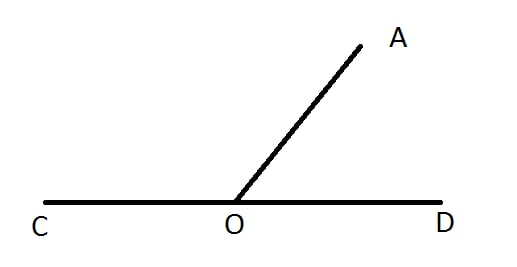
\includegraphics[width=0.7\linewidth]{pics/G51M4C8-1.jpg}
	 \end{minipage}
 	\begin{center}
 		Биссектриса угла --- луч, исходящий из вершины угла и делящий этот угол на два равных угла.
 	\end{center}
 	\item \( \angle ACB \) равен \( 50\degree \). Провели биссектрису \( CO \). Чему равен \( \angle ACO \)?
 	\item \( \angle KLM \) равен \( 140\degree \). Провели луч \( LO \). Угол \( KLO=40\degree \). Чему равен \( \angle OLM \)?
 	\item 
 	\begin{minipage}[t]{0.73\linewidth}
 		Найдите все углы
 	\end{minipage}
 	\hspace{0.03\linewidth}
 	\begin{minipage}[c]{0.24\linewidth}
 		\includegraphics[width=0.7\linewidth]{pics/G51M4C8-2.jpg}
 	\end{minipage}
	\end{listofex}
\end{class}
%===============>>  Проверочная работа  <<===============
%
\begin{exam}
	\title{Проверочная работа}
	\begin{listofex}
		\item Вычислите:
		\begin{enumcols}[itemcolumns=4]
			\item \( 4+\dfrac{1}{2} \)
			\item \( \dfrac{2}{5}+\dfrac{9}{10} \)
			\item \( \mfrac{5}{3}{4}-\mfrac{1}{3}{8} \)
			\item \( \dfrac{97}{100}-\dfrac{3}{50} \)
		\end{enumcols}
		\item Вычислите:
		\begin{enumcols}[itemcolumns=4]
			\item \( \dfrac{2}{3}\cdot\dfrac{5}{6} \)
			\item \( \dfrac{12}{63}\cdot\dfrac{21}{24} \)
			\item \( \mfrac{5}{1}{2}\cdot\mfrac{3}{2}{7} \)
			\item \( \mfrac{100}{1}{20}\cdot\mfrac{2}{198}{2001} \)
		\end{enumcols}
			\item Являются ли следующие числа взаимно обратными? Почему?
			\begin{enumcols}[itemcolumns=6]
				\item \( 7 \) и \( \dfrac{1}{7} \)
				\item \( \dfrac{6}{7} \) и \( \dfrac{14}{12} \)
				\item \( \dfrac{1}{2} \) и \( \dfrac{2}{4} \)
				\item \( \mfrac{2}{1}{6} \) и \( \dfrac{6}{13} \)
				\item \( \mfrac{1}{4}{5} \) и \( \dfrac{25}{45} \)
				\item \( \mfrac{7}{1}{2} \) и \( \mfrac{2}{1}{7} \)
			\end{enumcols}			
			\item Сколько времени затратил пешеход, который прошёл \( \mfrac{5}{1}{2} \) км со скоростью \( \mfrac{4}{2}{5} \) км/ч?
			\item Вычислить: \( \left( \cfrac{3}{20}\cdot\left( \cfrac{7}{12}-\cfrac{1}{2} \right)+\cfrac{79}{80} \right):\left( \cfrac{13}{24}:\left( \cfrac{7}{12}+\cfrac{1}{2} \right)-\cfrac{1}{4} \right) \)
	\end{listofex}
\end{exam}
		\newpage
		\title{Консультация}
	\begin{listofex}
			\item Вычислить:
				\begin{tasks}(2)
					\task \( 312:5 \)
					\task \( 500:18 \)
					\task \( 2808:78 \)
					\task \( 26031:400 \)
				\end{tasks}	
			\item Найдите неизвестное делимое в выражении:
			\begin{tasks}(2)
				\task \( x:17=18 \) (остаток \( 4 \))
				\task \( x:4=9 \) (остаток \( 2 \))
				\task \( b:2=7 \) (остаток \( 1 \))
				\task \( y:5=6 \) (остаток \( 3 \))
			\end{tasks}	
			\item Настя раскладывает свои карандаши по пеналам. Карандашей у Насти \( 210 \) штук, а отделений в пенале, в которое помещается только один карандаш --- \( 26 \). Сколько пеналов потребуется Насте, чтобы убрать все карандаши?
			\item В математической школе \( " \)Симметрия\( " \) в группе \( 5-1 \) каждое занятие пьют чай. Учеников в группе четверо, а также есть один преподаватель, каждый человек использует один пакетик чая. В неделю у группы \( 5-1 \) по \( 2 \) занятия. В одной упаковке уложено \( 25 \) пакетиков. Сколько упаковок чая потребуется, чтобы каждое занятие в течение месяца "чаёвничать"?
			\item На сколько остаток от деления \( 120 \) на \( 11 \) больше остатка от деления \( 65 \) на \( 4 \)?
			\item На сколько нужно увеличить число \( 37 \), чтобы остаток от получившегося числа на \( 5 \) был равен \( 4 \)?
			\item Разбейте число \( 10 \) на два числа так, чтобы при делении каждого числа на \( 3 \), остатки были у обоих были равны \( 2 \).
			\item Товарный поезд прошёл \( \mfrac{31}{1}{2} \) км за \( \dfrac{3}{4} \) часа. Какова его скорость?
			\item Куплено \( \mfrac{7}{1}{2} \) м ткани по \( \mfrac{5}{1}{2} \) руб. и \( 5 \) м по \( \mfrac{3}{3}{4} \) за \( 1 \) м. Сколько стоит вся покупка?
	\end{listofex}